%% LyX 2.0.5.1 created this file.  For more info, see http://www.lyx.org/.
%% Do not edit unless you really know what you are doing.
%\documentclass[12pt,english]{report}
%\usepackage{mathptmx}
%\renewcommand{\familydefault}{\rmdefault}
%\usepackage[T1]{fontenc}
%\usepackage[latin9]{inputenc}
%\usepackage[a4paper]{geometry}
%\setcounter{secnumdepth}{2} % Changed from 3 to 2. 0-chapter 1-section 2-subsection 
%\setcounter{tocdepth}{2} % Changed from 3 to 2. 0-chapter 1-section 2-subsection 
%\setlength{\parskip}{\medskipamount}
%\setlength{\parindent}{0pt}
%\usepackage{verbatim}
%\usepackage{pdfpages}
%\usepackage{graphicx}
%\usepackage{subfig} %% This package has to be here
%\usepackage{setspace}
%\usepackage{arabtex}
%\usepackage[numbers]{natbib}
%\usepackage{nomencl}
%\usepackage{amsthm}
%\usepackage{amsmath}
%\usepackage{amsfonts}
%\usepackage{paralist}
%\usepackage{etoolbox}
%\newtoggle{edit-mode}
%\toggletrue{edit-mode}  
%%%\toggletrue{edit-mode}
%\iftoggle{edit-mode}{
%\geometry{verbose,tmargin=2cm,bmargin=2cm,lmargin=2cm,rmargin=6cm,headheight=1cm,headsep=1cm,footskip=1cm, marginparwidth=5cm}
%}{
%\geometry{verbose,tmargin=2cm,bmargin=2cm,lmargin=2cm,rmargin=2cm,headheight=1cm,headsep=1cm,footskip=1cm}
%}
%
%\makenomenclature
%
%%% Theorem Styles
%\newtheorem{theorem}{Theorem}[section]
%%% Definition Styles
%\theoremstyle{definition}
%\newtheorem{definition}{Definition}[section]
%\newtheorem{example}{Example}[section]
%\theoremstyle{remark}
%\newtheorem{remark}{Remark}
%
%\usepackage[linesnumbered]{algorithm2e}
%
%\begin{document}

\chapter{Data Collection}
\label{chap:data_collection}

\section{The ADAB Database}
\label{sec:adab_database}

\iftoggle{edit-mode}{\hspace{0pt}\marginpar{The data importance}}{}
The quality of the collected data and it's amount is a fundamental aspect of any supervised learning technique.
It is used for learning, validation and testing and has a critical effect on the system performance.

\iftoggle{edit-mode}{\hspace{0pt}\marginpar{Data representation Definition}}{}
On-line handwriting data is commonly a digitized representation of the pen movement. 
It may contain sequential information about position, velocity, acceleration, pressure, or even angle and orientation of the pen as a function of time. 
However, the most basic and used property is the position of the pen. 
Although the sampling of the pen position is done in a constant time intervals, in most cases, HWR system do not use the temporal information but only consider the ordered set of sequential pen position. 

\iftoggle{edit-mode}{\hspace{0pt}\marginpar{Lack of databases}}{}
Unfortunately, there is only a single medium size public corpus of on-line handwriting.
The reason for this lack in database may be attributed to the fact that the major work done on Arabic handwriting recognition, focused on recognizing off-line script \cite{plamondon2000online}. 
Another reason is that the most of the work in on-line script recognition field is done for isolated characters such as letters, digits and symbols \cite{al2011online}.

\iftoggle{edit-mode}{\hspace{0pt}\marginpar{Information about the ADAB database}}{}
In this work we have chosen to use the ADAB (Arabic DAtaBase) database.
The ADAB database is de-facto a standard in the on-line Arabic handwriting recognition field.
It was developed to advance the research and development of Arabic on-line handwritten text recognition systems \cite{el2011line}.
It is freely available and consists of more than 20k Arabic handwritten words scribed by more than 170 different writers.
The samples are words that were taken from the 937 Tunisian town/village names, and for this reason, a sample can contain more than a word.
The information saved in the database is the strokes information in an XML file format. 
Each stroke, represented as a node in the XML, contains the sequence of $(x,y)$ coordinates of the pen position expands from the pen-down event to the corresponding pen-up event, as can be seen in Figure \ref{fig:adab_inkml}.
In addition to the strokes positional information, the database contains several properties related to the equipment used to obtain the data and the writer's information, as well as the plot image of the word trajectory as shown in Figure \ref{fig:sample_parts}.

\begin{figure}
\centering
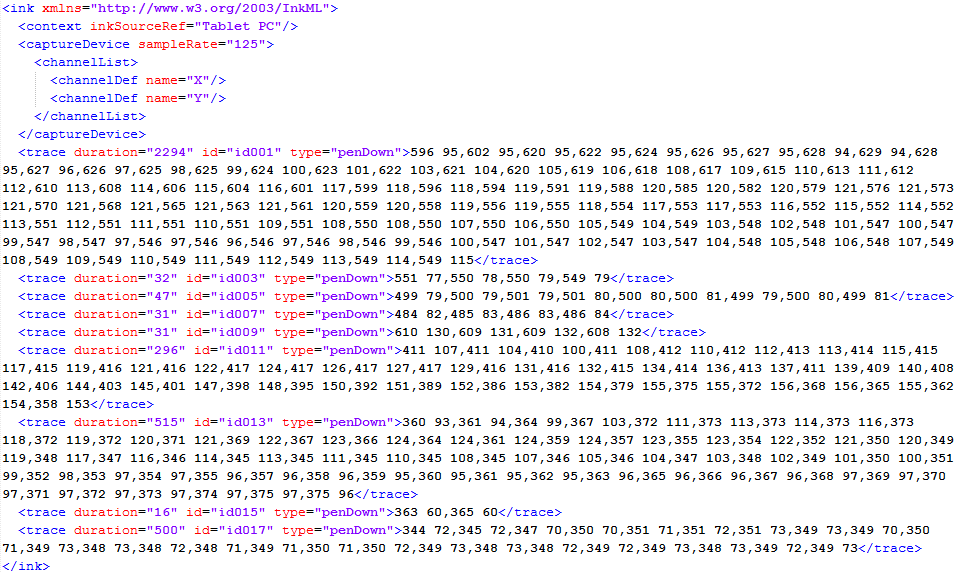
\includegraphics[width=1\textwidth]{./figures/adab_inkml}
\caption{Trajectory information of a city name sample.}
\label{fig:adab_inkml}
\end{figure}

\begin{figure}
\centering
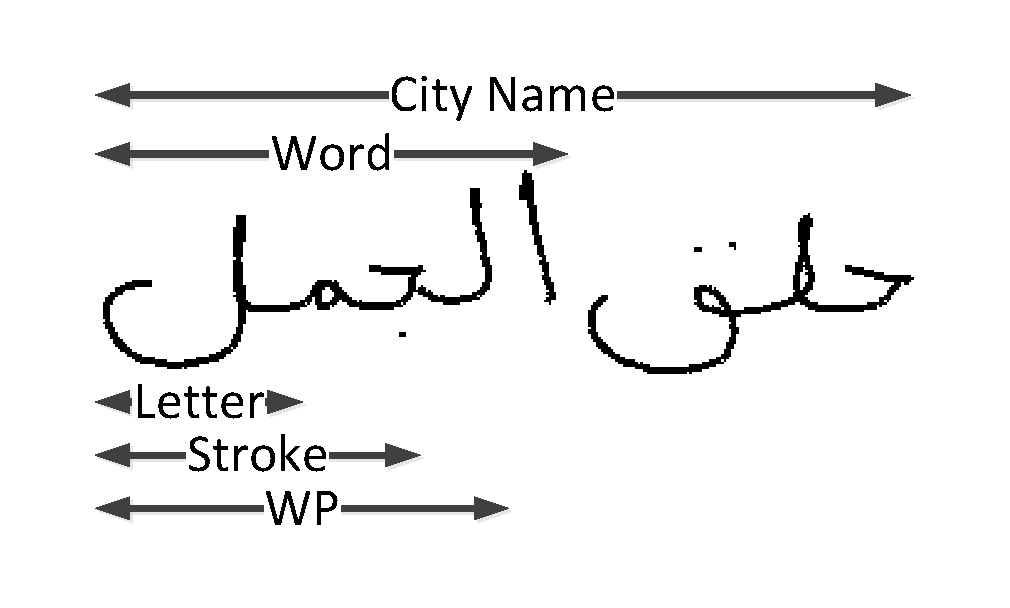
\includegraphics[width=0.65\textwidth]{./figures/sample_parts}
\caption{Visual demonstration of a test sample parts.}
\label{fig:sample_parts}
\end{figure}


%%%%%%%%%%%%%%%%%%%%%%%%%%%%%%%%%%%%%%%%%%%%%%%%%%%%%%%
\newpage{}
%%%%%%%%%%%%%%%%%%%%%%%%%%%%%%%%%%%%%%%%%%%%%%%%%%%%%%%

\section{Letters Extraction}
\label{sec:letters_extraction}

\iftoggle{edit-mode}{\hspace{0pt}\marginpar{The missing information}}{}
In order to obtain letter samples required for the training of our letters classifier, manual segmentation of the strokes provided in the ADAB database was required.
However, no mapping between strokes and letters was provided, thus, extra work was needed to add this information to the database so that it could be used as letters samples source and also as a ground-truth for for validating our segmentation algorithm accuracy.

\iftoggle{edit-mode}{\hspace{0pt}\marginpar{How is the data available}}{}
The challenge was to match each word part to each stroke, and then manually segment each sequence which describes a word-part to letters (subsequences). Another problem we faced was that automatically corresponding each stroke to each word-part was not easy.

\iftoggle{edit-mode}{\hspace{0pt}\marginpar{Letters extraction method}}{}
To extract this additional information, we have created a system that reads the samples from the ADAB database, and employs the skills of a human expert to segment the samples and relate each stroke to the corresponding letter in the WP. 

\iftoggle{edit-mode}{\hspace{0pt}\marginpar{Additional strokes detection and removal}}{}
Since additional strokes are not our interest in the segmentation process, the system has automatically filtered out additional strokes. 
The detection of delayed strokes is performed based on their size and the area of their bounding box. 
However, in order to avoid unintentionally removing main body of small letters, we preset a low high threshold. 
Thus, the human expert had to filter out additional strokes manually that could not be identified by the system as such.

\iftoggle{edit-mode}{\hspace{0pt}\marginpar{The output structure}}{}
The resulted information was saved in an XML file for each word sample. See figure \ref{fig:adab_segmented_xml}.
We have manually segmented ~16k samples which consisted about ~40k strokes. 

\begin{figure}[h]
\centering
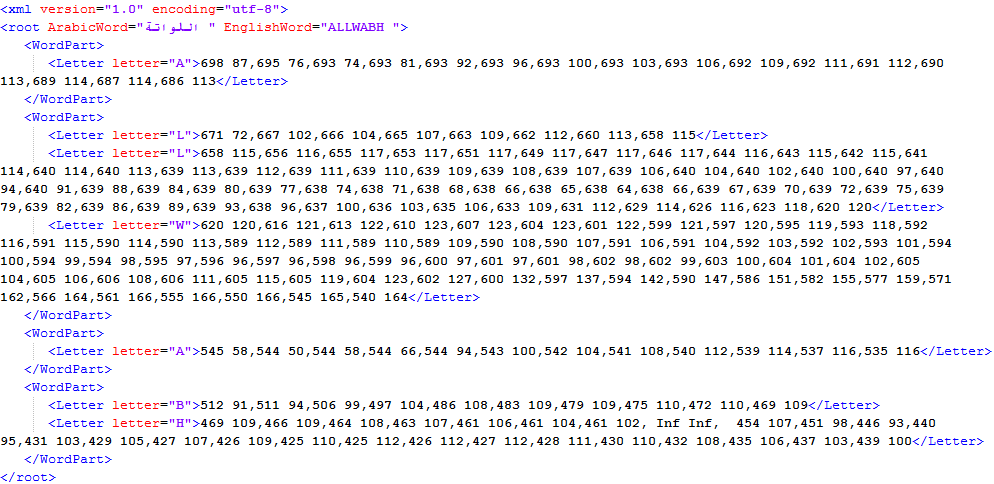
\includegraphics[width=1\textwidth]{./figures/adab_segmented_xml}
\caption{Trajectory information of a city name sample.}
\label{fig:adab_segmented_xml}
\end{figure}

%\bibliographystyle{plainnat}
%\bibliography{references}
%\end{document}

%\begin{itemize}
%\item Discuss the letters extraction from the adab database.
%\item Describe the system developed by Wajdi
%\item mention that the number of samples per class is different from letter to letter
%\item see "Removing delayed strokes" section in \cite{jaeger2001online}
%\item extract information from the paper written by raid.
%\item add images of the segmentation system.
%\item add an image of the output xml.
%\end{itemize}
